\documentclass[aspectratio=169]{beamer}
\usetheme{metropolis}

%------------------------------------------------
% Pacotes
\usepackage[T1]{fontenc}
\usepackage[utf8]{inputenc}
\usepackage[brazil]{babel}
\usepackage{graphicx}
\usepackage{amsmath}
\usepackage{booktabs}

%------------------------------------------------
% Meta
\title{Visualizing Population Dynamics in Neuroevolutionary Weight Spaces With Aligned Projections and Vector Fields}
\author{Fernando Souza da Silveira \\ Orientador: Prof. Dr. Bruno Iochins Grisci}
\institute{PPGC -- Instituto de Informática -- UFRGS}
\date{Dezembro de 2025}

% Logos para agradecimentos
\newcommand{\thankyoulogos}{
  
\includegraphics[height=0.9cm]{lab.png}
  
\includegraphics[height=0.9cm]{inf.jpg}
  
\includegraphics[height=0.9cm]{ufrgs2.jpg}
  
\includegraphics[height=0.9cm]{fapergs.jpg}
  
\includegraphics[height=0.9cm]{serra.png}
}

\begin{document}

\begin{frame}
  \titlepage
\end{frame}

% CONTEXTO INICIAL 
\begin{frame}{Redes Neurais}

\footnotesize
\begin{itemize}
  \item Uma rede neural é um modelo que transforma entradas em saídas.
  \item Ela possui parâmetros internos.
  \item Esses parâmetros controlam como a informação flui na rede.
  \item Os parâmetros internos são chamados de pesos e bias.
  \item O comportamento da rede depende desses parâmetros.
  \item Treinar uma rede significa ajustar esses valores.
\end{itemize}

\vspace{0.2cm}
\centering
\textit{Neste trabalho, o foco está nos parâmetros da rede.}

\vspace{0.15cm}
\centering
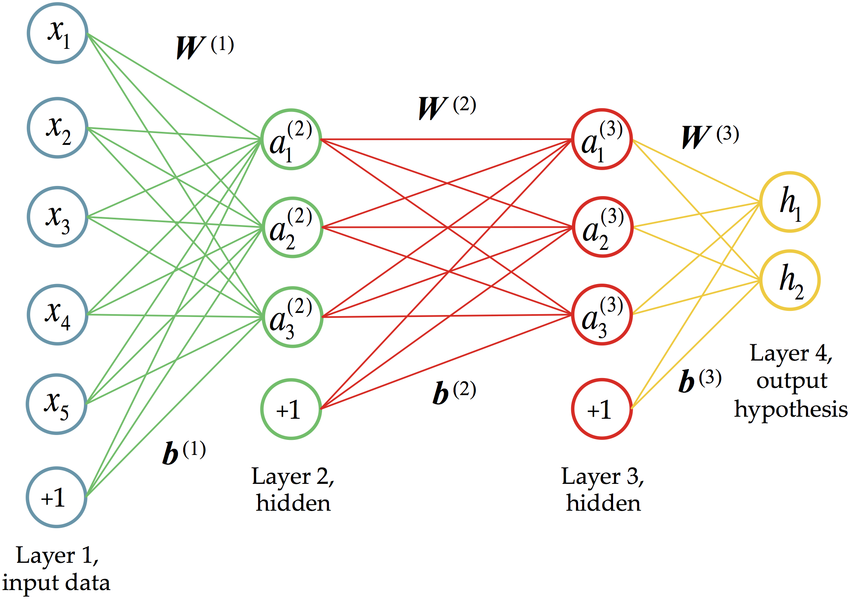
\includegraphics[
  width=0.72\linewidth,
  height=0.40\textheight,
  keepaspectratio
]{nn_mlp_theta.png}

\end{frame}

\begin{frame}{Algoritmos Evolutivos}

\begin{itemize}
  \item Algoritmos inspirados no processo de evolução natural.
  \item Trabalham com uma \textbf{população} de soluções.
  \item A cada iteração:
  \begin{itemize}
    \item avaliam as soluções,
    \item mantêm as melhores,
    \item geram novas variações.
  \end{itemize}
\end{itemize}

\vspace{0.15cm}
\centering
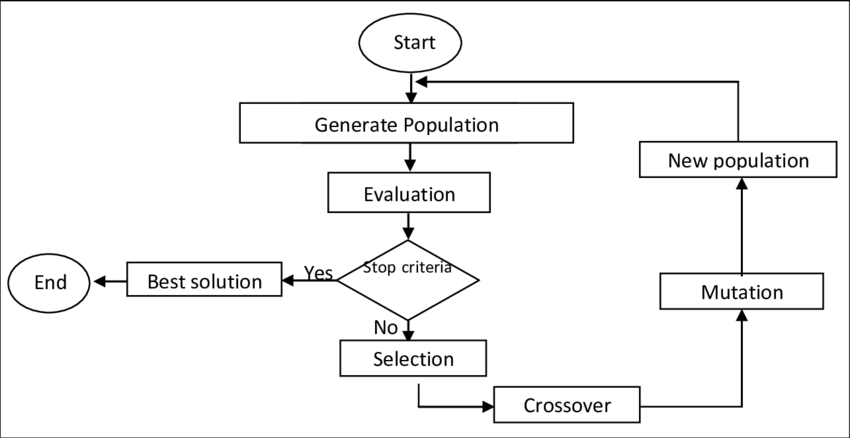
\includegraphics[
  width=0.85\linewidth,
  height=0.5\textheight,
  keepaspectratio
]{ga_flow.png}

\end{frame}

\begin{frame}{Neuroevolução}
\begin{itemize}
  \item Neuroevolução aplica algoritmos evolutivos ao treinamento de redes neurais.
  \item Cada indivíduo da população $\leftrightarrow$ uma rede (parâmetros $\theta$).
  \item Otimização ocorre diretamente no \textbf{espaço de pesos}.
\end{itemize}

\vspace{0.2cm}
\centering
% IMAGEM SUGERIDA: loop "Evaluate -> Select -> Mutate" com ícones de redes/indivíduos (neuroevolution loop).
% Você já tem uma figura compatível: neuroevolution_loop.png
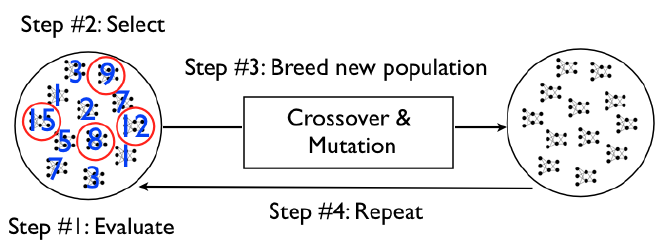
\includegraphics[width=0.70\linewidth]{neuroevolution_loop.png}
\end{frame}

%PROBLEMA E SOLUÇÃO

\begin{frame}{Motivação}

\begin{itemize}
  \item Neuroevolução gera uma \textbf{população} de redes a cada geração.
  \item Na prática, a análise costuma se limitar a métricas escalares
        (ex.: fitness médio ou máximo).
  \item Essas métricas não revelam:
  \begin{itemize}
    \item como a população se organiza,
    \item como os pesos evoluem,
    \item nem padrões dinâmicos ao longo do tempo.
  \end{itemize}
  \item Falta suporte para analisar a \textbf{dinâmica populacional no espaço de pesos}.
\end{itemize}

\end{frame}

\begin{frame}{Contribuição}

\begin{itemize}
  \item Proposta de uma abordagem visual para analisar
        \textbf{dinâmicas populacionais no espaço de pesos}.
  \item Uso de:
  \begin{itemize}
    \item projeções dimensionais (UMAP),
    \item alinhamento temporal entre gerações,
    \item campos vetoriais para resumir tendências.
  \end{itemize}
  \item A abordagem permite:
  \begin{itemize}
    \item observar deslocamentos coletivos,
    \item identificar padrões de convergência ou dispersão,
    \item complementar métricas escalares tradicionais.
  \end{itemize}
\end{itemize}

\end{frame}

%INSPIRAÇÃO/REF

\begin{frame}{Trabalhos Relacionados}

\begin{columns}[T,onlytextwidth]

%-------------------------
\column{0.45\textwidth}
\centering
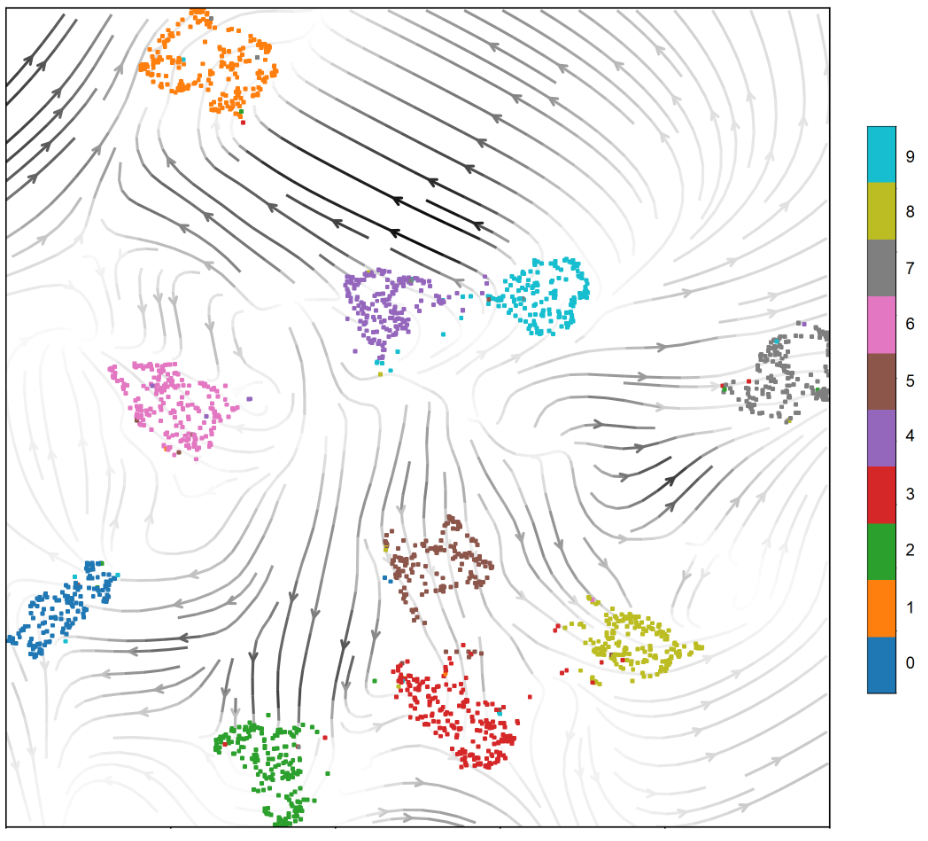
\includegraphics[
  width=\linewidth,
  height=0.68\textheight,
  keepaspectratio
]{cantareira.png}

\vspace{0.1cm}
\scriptsize
\textit{Cantareira et al. (2020). Exploring Neural Network Hidden Layer Activity Using Vector Fields.}

%-------------------------
\column{0.55\textwidth}
\begin{itemize}
  \item Abordagem visual para analisar \textbf{dinâmicas internas} em redes neurais.
  \item Foco na evolução de \textbf{ativações de camadas ocultas} ao longo do treinamento.
  \item Técnicas centrais:
  \begin{itemize}
    \item projeções dimensionais alinhadas (ex.: UMAP),
    \item trajetórias temporais,
    \item campos vetoriais para representar o fluxo global.
  \end{itemize}
\end{itemize}

\end{columns}

\end{frame}

\begin{frame}{UMAP}

\begin{itemize}
  \item UMAP (\textit{Uniform Manifold Approximation and Projection})
        é um método de \textbf{redução de dimensionalidade}.
  \item Projeta dados de alta dimensão para 2D preservando
        \textbf{relações de vizinhança}.
  \item Pontos próximos no espaço original tendem a permanecer próximos
        na projeção.
  \item Permite visualizar estruturas, agrupamentos e transições
        em dados complexos.
\end{itemize}

\vspace{0.2cm}
\centering
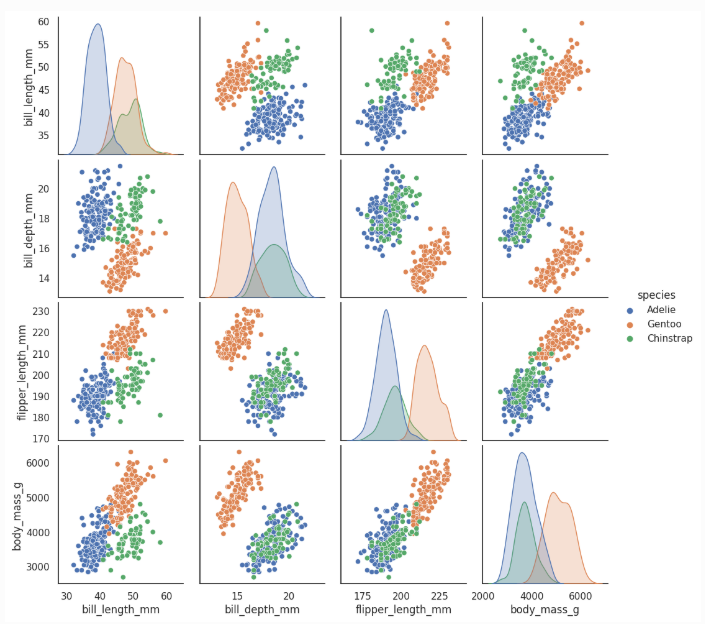
\includegraphics[
  width=0.75\linewidth,
  height=0.45\textheight,
  keepaspectratio
]{umap_explanation.png}

\vspace{0.1cm}
\footnotesize
\textit{Neste trabalho, UMAP é usado para projetar populações de pesos
em um espaço visual interpretável.}

\end{frame}

%DATASET
\begin{frame}{Dataset do Experimento — Make Moons}

\begin{itemize}
  \item Dataset sintético clássico para \textbf{classificação não linear}.
  \item Duas classes em formato de “meias-luas”.
  \item Usado para avaliar a capacidade de separação da rede.
  \item Configuração:
  \begin{itemize}
    \item 400 amostras,
    \item ruído \texttt{noise = 0.25},
    \item dados padronizados com \texttt{StandardScaler}.
  \end{itemize}
\end{itemize}

\vspace{0.15cm}
\centering
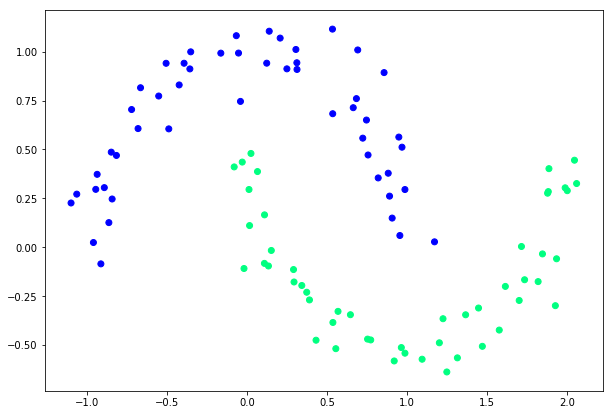
\includegraphics[
  width=0.75\linewidth,
  height=0.45\textheight,
  keepaspectratio
]{makemoons.png}

\end{frame}


% REDE
\begin{frame}{Arquitetura da Rede Neural (MLP)}

\begin{itemize}
  \item Rede com duas entradas, uma camada intermediária e uma saída.
  \item Camada intermediária: $H$ neurônios (tamanho escolhido no app), faz uma transformação não linear.
  \item Saída: 1 neurônio que devolve um valor entre 0 e 1 para classificar.
  \item Só ajustamos os pesos das conexões durante a neuroevolução; a forma da rede continua a mesma.
\end{itemize}

\end{frame}

%ALGO
\begin{frame}{Algoritmo Neuroevolutivo}

\begin{itemize}
  \item Tipo: Evolution strategy (ES) (elitismo + mutação gaussiana, sem crossover).
  \item Começamos com uma população de redes iniciais aleatórias (arquitetura fixa).
  \item Em cada geração:
  \begin{itemize}
    \item avaliamos o desempenho de cada rede,
    \item mantemos as melhores (elitismo),
    \item geramos o restante aplicando pequenas mutações aleatórias nos pesos (ruído gaussiano).
  \end{itemize}
  \item Repetimos por $G$ gerações; não há cruzamento, apenas seleção + mutação.
  \item O app permite ajustar tamanho da população, número de gerações, taxa de mutação e seed.
\end{itemize}

\end{frame}


%SNAPSHOT ATÉ AGORA

\begin{frame}{Snapshot: Configurações Atuais}

\begin{itemize}
  \item \textbf{Dataset}: make\_moons com 400 amostras, ruído 0{,}25, padronizado, seed configurável.
  \item \textbf{Rede (MLP)}: 2 entradas → $H$ neurônios na camada oculta (tanh, sem bias) → 1 saída sigmóide (binária); $H$ ajustado no app.
  \item \textbf{Algoritmo neuroevolutivo}: estratégia evolutiva simples (elitismo + mutação gaussiana, sem crossover), população e gerações configuráveis; parâmetros chave: tamanho da população, nº de gerações, taxa de mutação, seed.
\end{itemize}

\end{frame}


\begin{frame}{Pipeline Metodológico}
\begin{itemize}
  \item Executar neuroevolução e registrar pesos.
  \item Projeção dimensional com UMAP.
  \item Alinhamento temporal.
  \item Campos vetoriais.
\end{itemize}
\end{frame}

\begin{frame}{Resultados - UMAP}
\centering
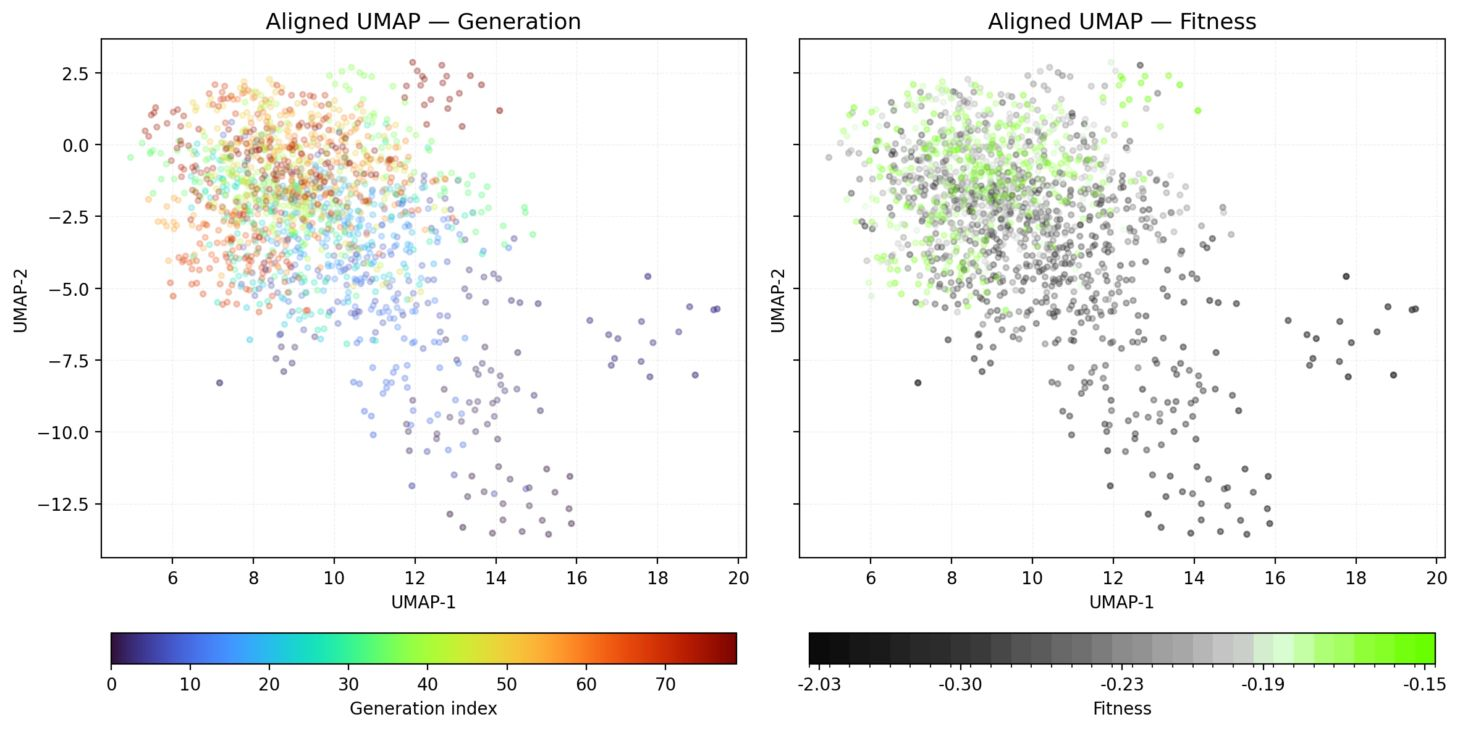
\includegraphics[width=0.9\linewidth]{aligned_umap.png}
\end{frame}

\begin{frame}{Resultados - Campo Vetorial}
\centering
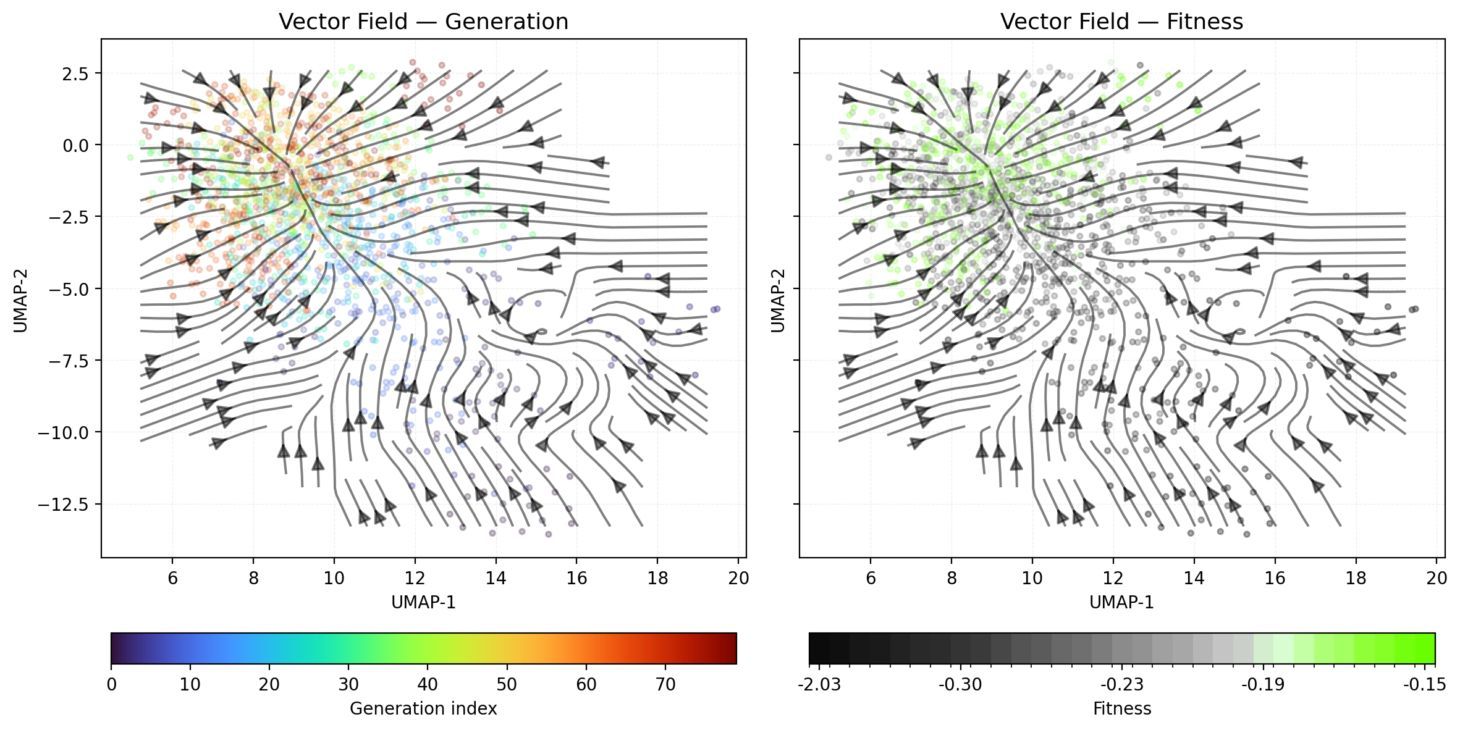
\includegraphics[width=0.9\linewidth]{vector_field.png}
\end{frame}

\begin{frame}{Implementação}
\begin{itemize}
  \item Linguagem: \textbf{Python}
  \item Bibliotecas:
  \begin{itemize}
    \item NumPy
    \item scikit-learn
    \item umap-learn
    \item Matplotlib, Plotly
    \item Streamlit
  \end{itemize}
\end{itemize}
\end{frame}

\begin{frame}{Ferramenta de Exploração Visual (Streamlit)}
\begin{itemize}
  \item Exploração visual interativa.
  \item Controle de geração, seed e parâmetros.
  \item Inspeção de indivíduos.
\end{itemize}

\centering
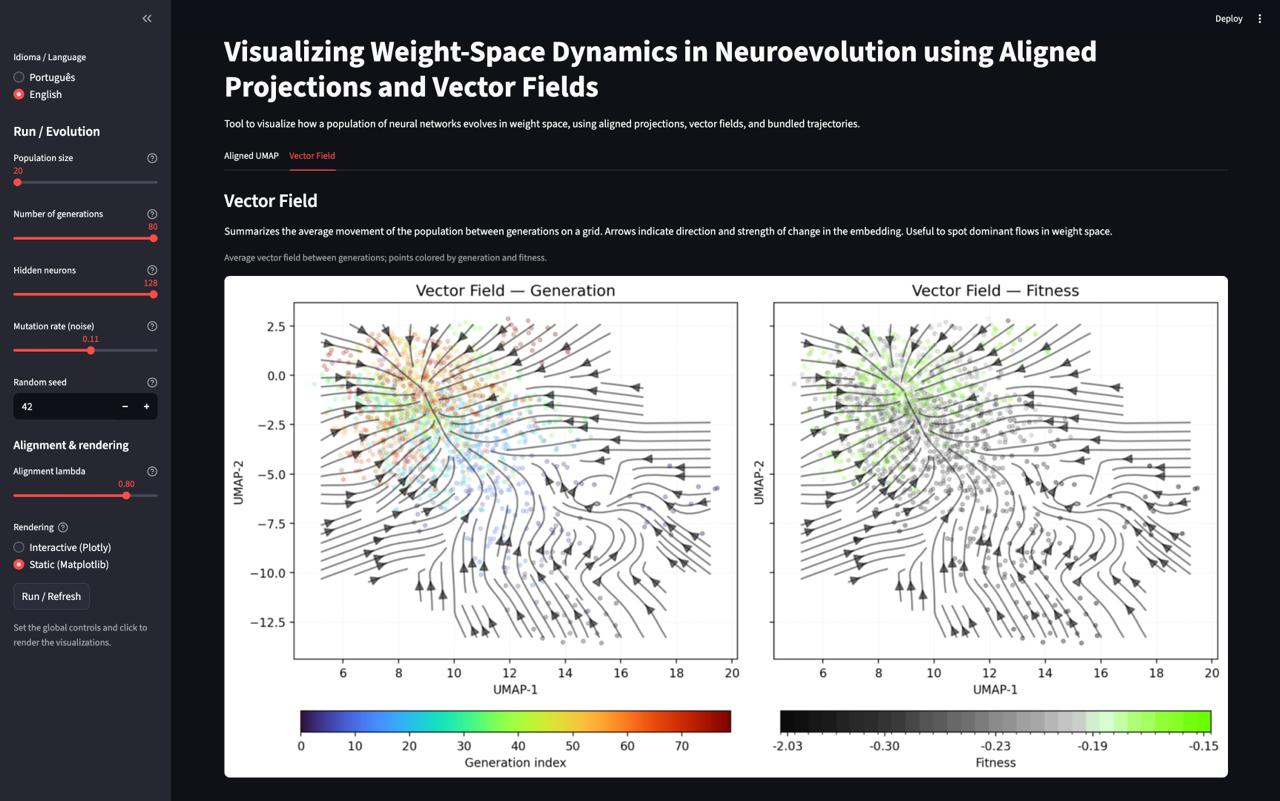
\includegraphics[width=0.75\linewidth]{streamlit.jpeg}
\end{frame}


\begin{frame}{Próximos Experimentos}
\begin{itemize}
  \item Gradiente de cores mais informativo.
  \item Fitness X Geração.
  \item Incluir Bias nos experimentos.
  \item Ativações X Pesos.
\end{itemize}
\end{frame}

\begin{frame}{Conclusão Parcial}

\begin{itemize}
  \item A abordagem proposta foi \textbf{implementada e validada} em um ambiente interativo.
  \item A ferramenta desenvolvida no \textbf{Streamlit} permite:
  \begin{itemize}
    \item explorar gerações da população,
    \item inspecionar indivíduos no embedding,
    \item visualizar campos vetoriais dinamicamente.
  \end{itemize}
  \item O pipeline é \textbf{modular} e facilmente adaptável a:
  \begin{itemize}
    \item novos datasets,
    \item diferentes arquiteturas,
    \item outros algoritmos neuroevolutivos.
  \end{itemize}
  \item A visualização revela padrões não observáveis
        apenas por métricas escalares.
\end{itemize}

\vspace{0.15cm}
\centering
\textit{Os resultados iniciais indicam viabilidade prática
e potencial de generalização da abordagem.}

\end{frame}



\begin{frame}[allowframebreaks]{Referências}
\footnotesize
\begin{thebibliography}{9}

\bibitem{cantareira2020}
Cantareira, G. D., Etemad, E., \& Paulovich, F. V. (2020).
\textit{Exploring Neural Network Hidden Layer Activity Using Vector Fields}.
Information, 11(9), 426.
\url{https://doi.org/10.3390/info11090426}

\bibitem{mcinnes2020}
McInnes, L., Healy, J., \& Melville, J. (2020).
\textit{UMAP: Uniform Manifold Approximation and Projection for Dimension Reduction}.
arXiv preprint arXiv:1802.03426.
\url{https://arxiv.org/abs/1802.03426}

\bibitem{bell2022}
Bell, O. (2022).
\textit{Applications of Gaussian mutation for self adaptation in evolutionary Genetic Algorithms}.
arXiv preprint arXiv:2201.00285.

\bibitem{stanley2019}
Stanley, K. O., Clune, J., Lehman, J., \& Miikkulainen, R. (2019).
\textit{Designing neural networks through neuroevolution}.
Nature Machine Intelligence, 1(1), 24--35.
\url{https://doi.org/10.1038/s42256-018-0006-z}

\bibitem{ashmore2015}
Ashmore, S. C. (2015).
\textit{Evaluating the Intrinsic Similarity between Neural Networks}.
Master’s Thesis, University of Arkansas.
\url{https://scholarworks.uark.edu/etd/1395}

\end{thebibliography}
\end{frame}

\begin{frame}{DEMO}
\centering

DEMO
\end{frame}



\begin{frame}{Agradecimentos}
\centering
\thankyoulogos

Perguntas?
\end{frame}

\appendix


\begin{frame}{EXTRAS/BACKUP}
\centering
EXTRAS/BACKUP
\end{frame}

\appendix





\begin{frame}{Neuroevolução vs. Backpropagation}

\begin{columns}[T,onlytextwidth]

%-------------------------
\column{0.48\textwidth}
\textbf{Backpropagation (SGD)}
\vspace{0.15cm}

\footnotesize
\begin{tabular}{c}
Parâmetros iniciais \\
$\downarrow$ \\
Gradiente \\
$\downarrow$ \\
Atualização \\
$\downarrow$ \\
\textbf{Trajetória única}
\end{tabular}

\vspace{0.2cm}
\begin{itemize}
  \item Atualizações guiadas por gradiente
  \item Uma única solução por execução
\end{itemize}

%-------------------------
\column{0.48\textwidth}
\textbf{Neuroevolução}
\vspace{0.15cm}

\footnotesize
\begin{tabular}{c}
População inicial \\
$\downarrow$ \\
Avaliação \\
$\downarrow$ \\
Seleção + mutação \\
$\downarrow$ \\
\textbf{População evolui}
\end{tabular}

\vspace{0.2cm}
\begin{itemize}
  \item Exploração paralela
  \item Mutações estocásticas
\end{itemize}

\end{columns}

\vspace{0.25cm}
\centering
\textit{Implicação: foco em dinâmica populacional, não em trajetórias individuais.}

\end{frame}



\begin{frame}{Relação com Cantareira et al. (2020)}

\begin{itemize}
  \item \textbf{Cantareira et al.}:
  \begin{itemize}
    \item analisam dinâmicas temporais de \textbf{ativações internas},
    \item em redes treinadas por gradiente,
    \item usando projeções alinhadas e campos vetoriais.
  \end{itemize}

  \item \textbf{Este trabalho}:
  \begin{itemize}
    \item analisa dinâmicas \textbf{populacionais} no espaço de pesos,
    \item em redes treinadas por \textbf{neuroevolução},
    \item adaptando essas técnicas ao espaço de parâmetros.
  \end{itemize}
\end{itemize}

\vspace{0.2cm}
\centering
\textit{Contribuição: transpor técnicas de visualização temporal
para o estudo de dinâmicas evolutivas no espaço de pesos.}

\end{frame}

\begin{frame}{Abordagem e Algoritmo de Neuroevolução}

\begin{itemize}
  \item Arquitetura da rede: \textbf{fixa} (MLP).
  \item Evolução aplicada exclusivamente aos \textbf{pesos}.
  \item Algoritmo: \textbf{algoritmo evolutivo populacional}, no estilo de
        \textbf{estratégias evolutivas}.
  \item Operadores: seleção elitista e mutação gaussiana.
\end{itemize}

\vspace{0.15cm}
\centering
\scriptsize
\begin{tabular}{c}
População de redes \\
↓ \\
Avaliação \\
↓ \\
Seleção elitista \\
↓ \\
Mutação gaussiana \\
↓ \\
Próxima geração
\end{tabular}

\vspace{0.15cm}
\centering

\end{frame}

\begin{frame}{Por que Visualizar o Espaço de Pesos?}

\begin{itemize}
  \item Os pesos determinam o comportamento da rede neural.
  \item Durante a neuroevolução, esses pesos \textbf{mudam ao longo do tempo}.
  \item Métricas escalares (como fitness) resumem o desempenho, mas \textbf{não mostram a dinâmica}.
  \item Redes com pesos próximos tendem a se comportar de forma semelhante.
\end{itemize}

\vspace{0.25cm}
\centering
\textit{Visualizar o espaço de pesos permite analisar a evolução da população, não apenas o resultado final.}

\end{frame}

\begin{frame}{Como o Campo Vetorial é Calculado}

\begin{itemize}
  \item Pega-se a posição de cada rede no UMAP na geração $t$ e na $t{+}1$ e calcula-se o vetor entre elas.
  \item Esses vetores são agrupados numa grade 2D; em cada célula, faz-se a média dos vetores que caem ali.
  \item Pode-se suavizar e ajustar o tamanho das setas, se necessário.
  \item O gráfico mostra as setas médias sobre os pontos, coloridos por geração ou fitness.
\end{itemize}

\end{frame}

\begin{frame}{Como alinhar o UMAP?}

\begin{itemize}
  \item Cada geração é projetada em 2D com UMAP.
  \item A 1ª projeção vira nosso “mapa de referência”.
  \item Nas gerações seguintes, a projeção é “puxada” em direção a esse mapa usando um fator $\lambda$ (alinhamento).
  \item O mapa de referência é atualizado como uma média das projeções alinhadas, mantendo tudo estável ao longo do tempo.
  \item Resultado: as nuvens não giram nem espelham aleatoriamente; dá para comparar gerações no mesmo “mapa”.
\end{itemize}

\end{frame}


\begin{frame}{Backup}

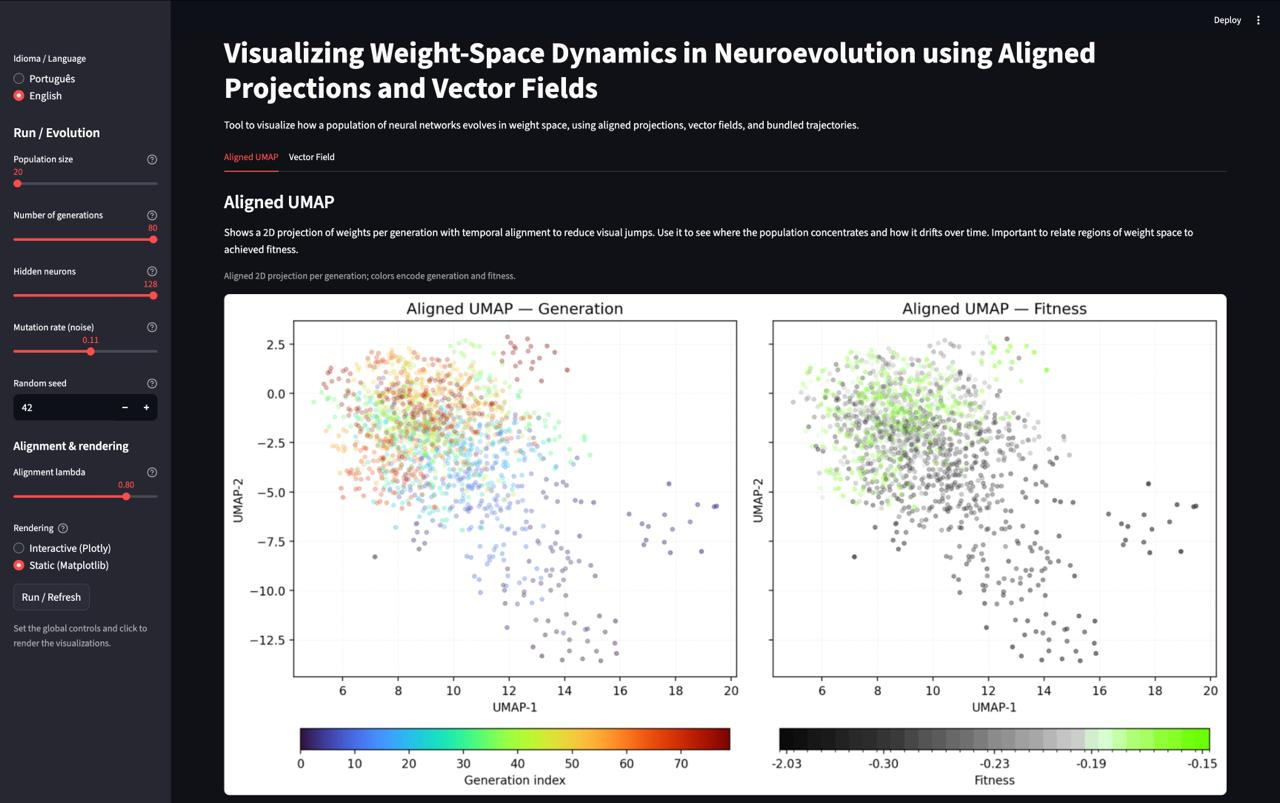
\includegraphics[width=0.9\linewidth]{streamlit2.jpeg}


\end{frame}

\begin{frame}{Backup}

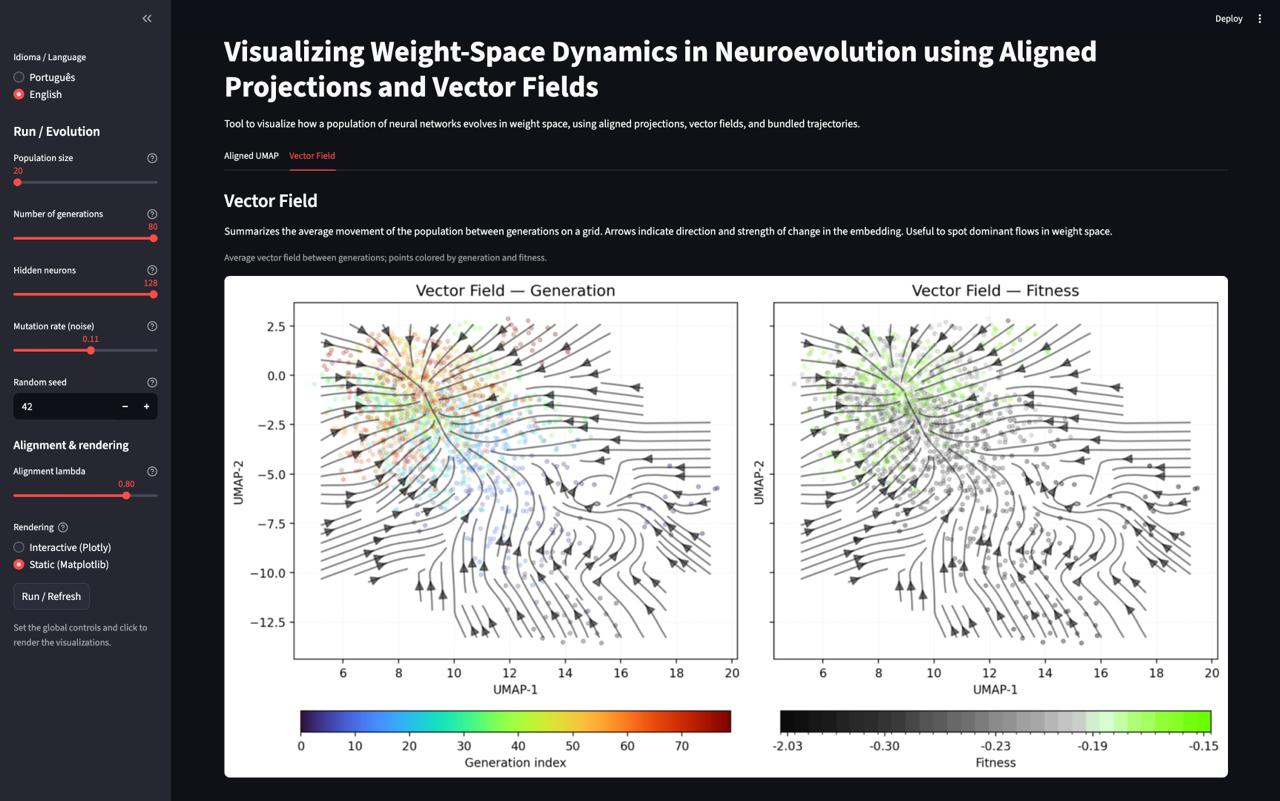
\includegraphics[width=0.9\linewidth]{streamlit.jpeg}

\end{frame}

\begin{frame}{Backup}

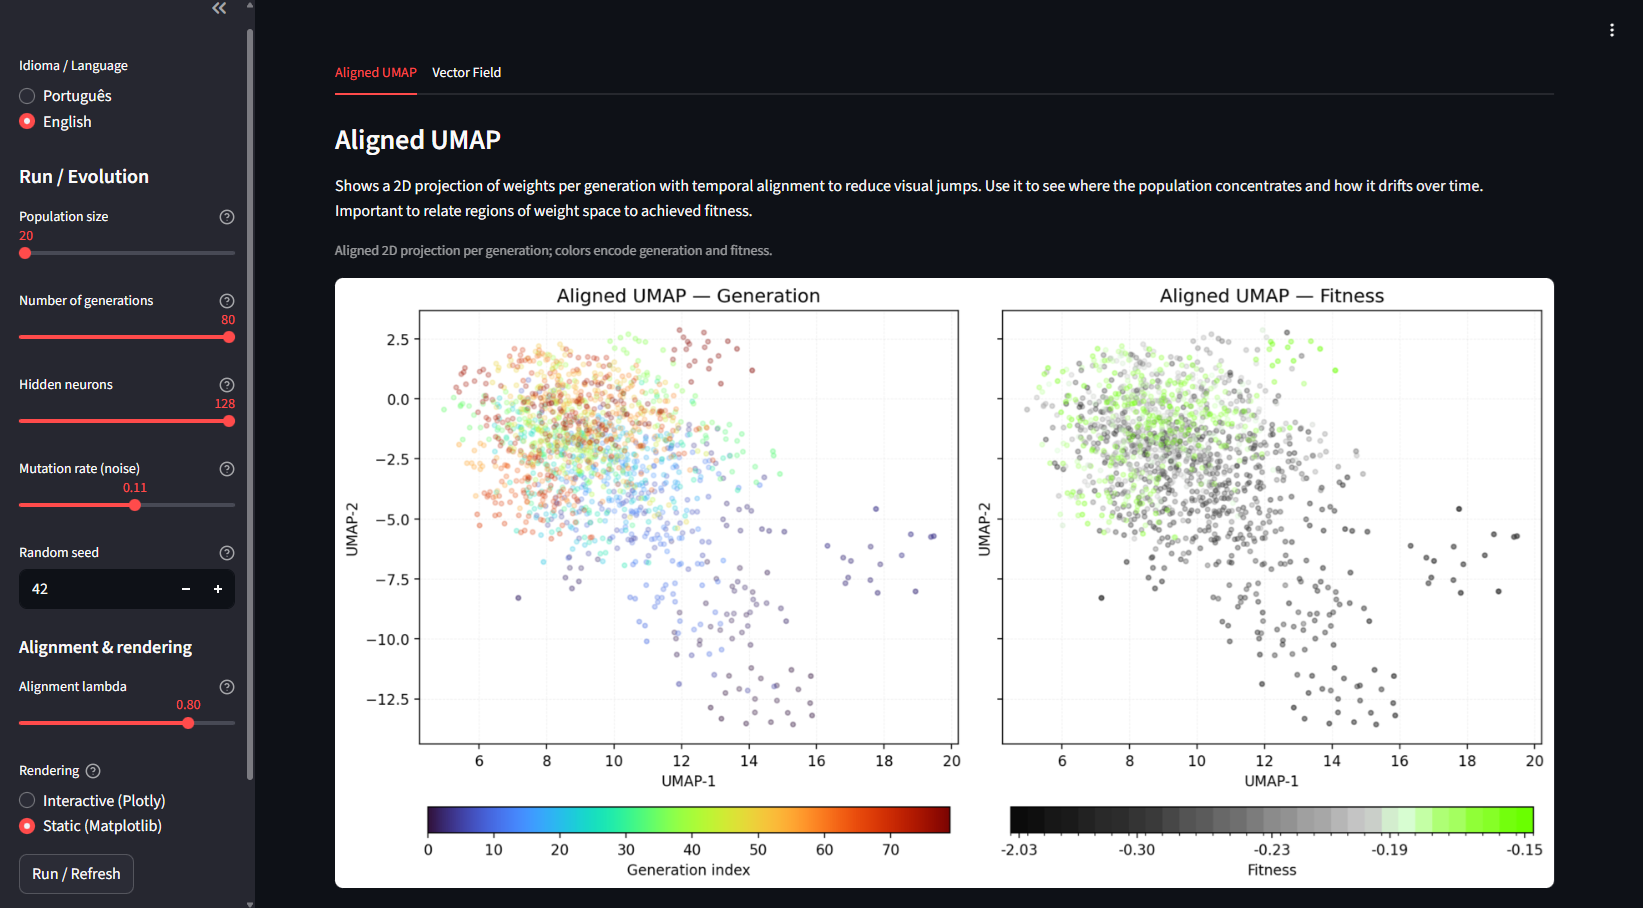
\includegraphics[width=0.9\linewidth]{streamlit3.png}

\end{frame}

\begin{frame}{Backup}

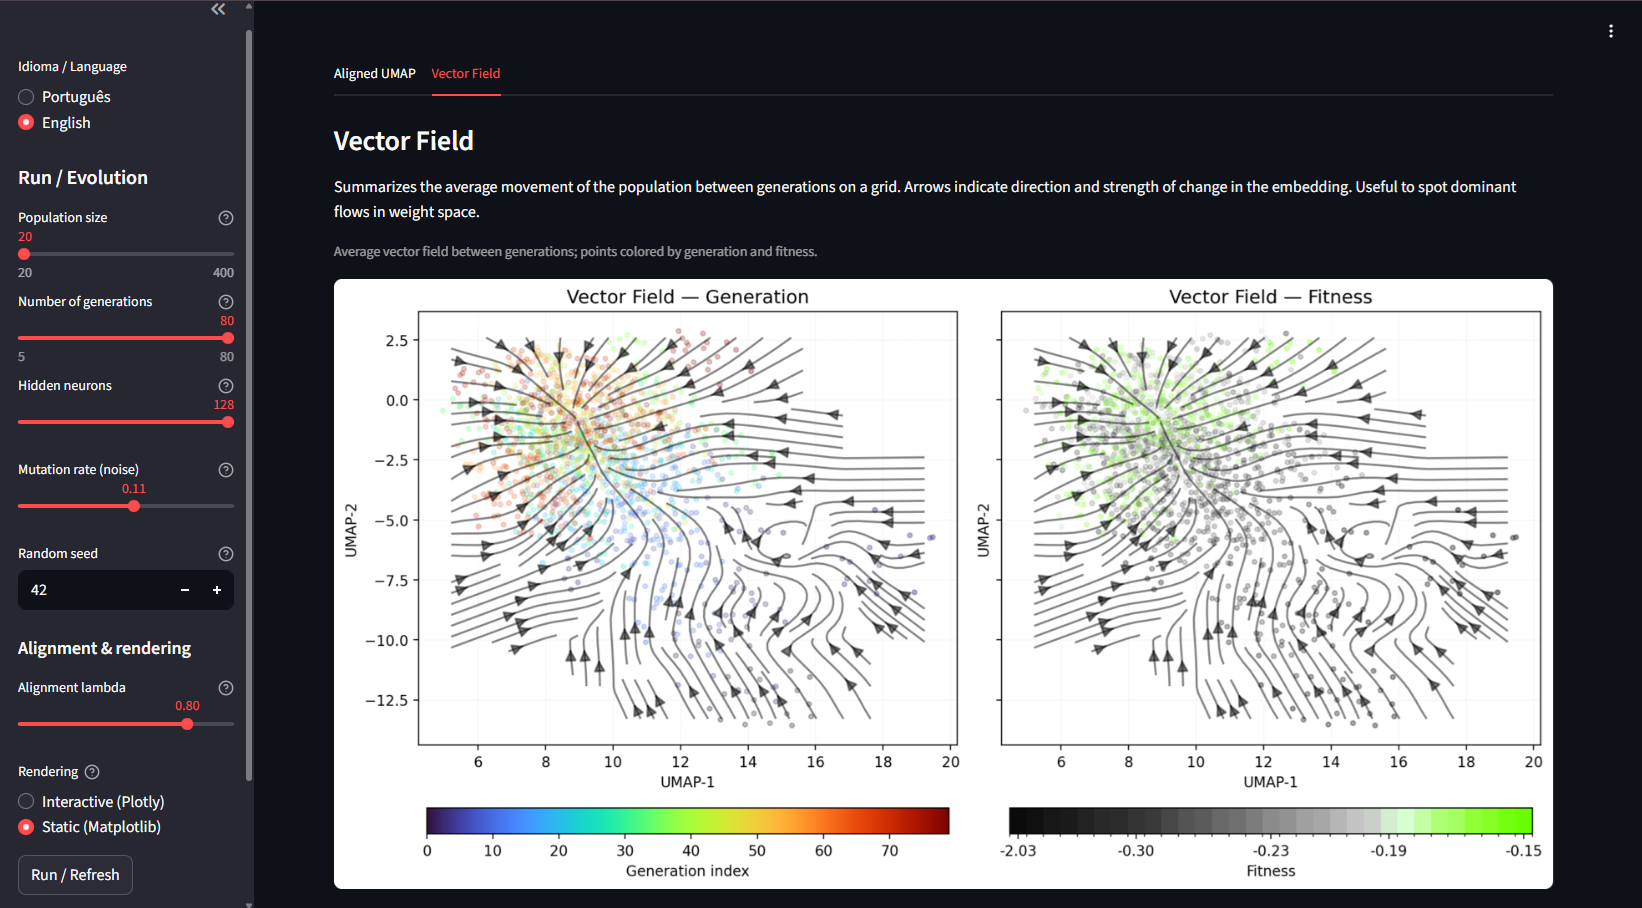
\includegraphics[width=0.9\linewidth]{streamlit4.png}

\end{frame}

\begin{frame}{Backup}

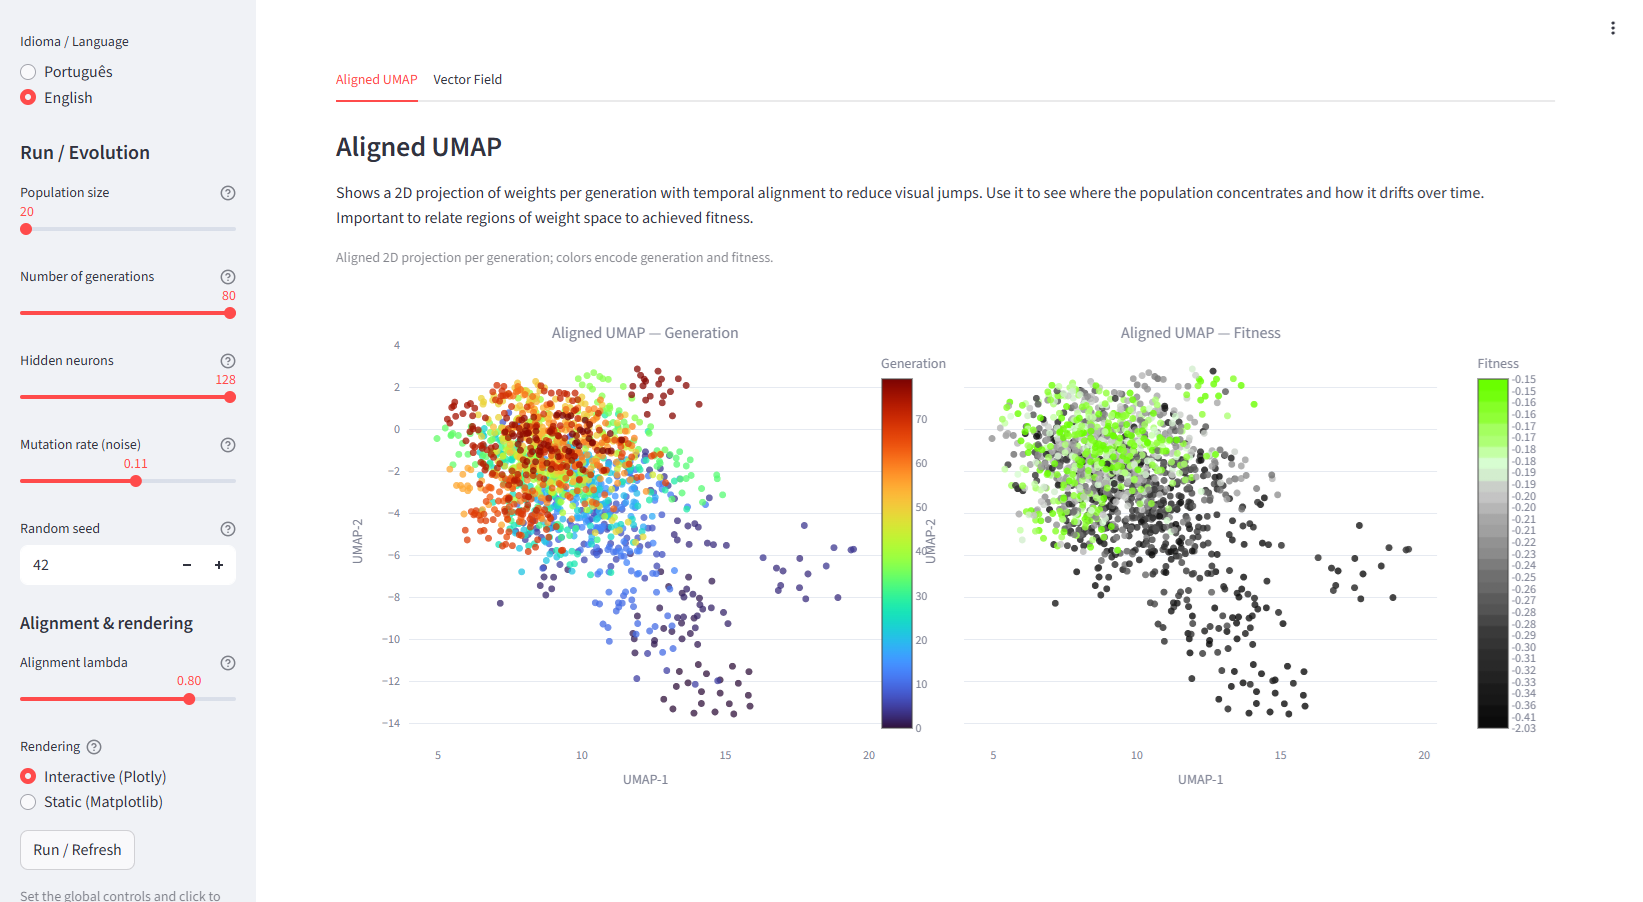
\includegraphics[width=0.9\linewidth]{streamlit5.png}

\end{frame}

\begin{frame}{Backup}

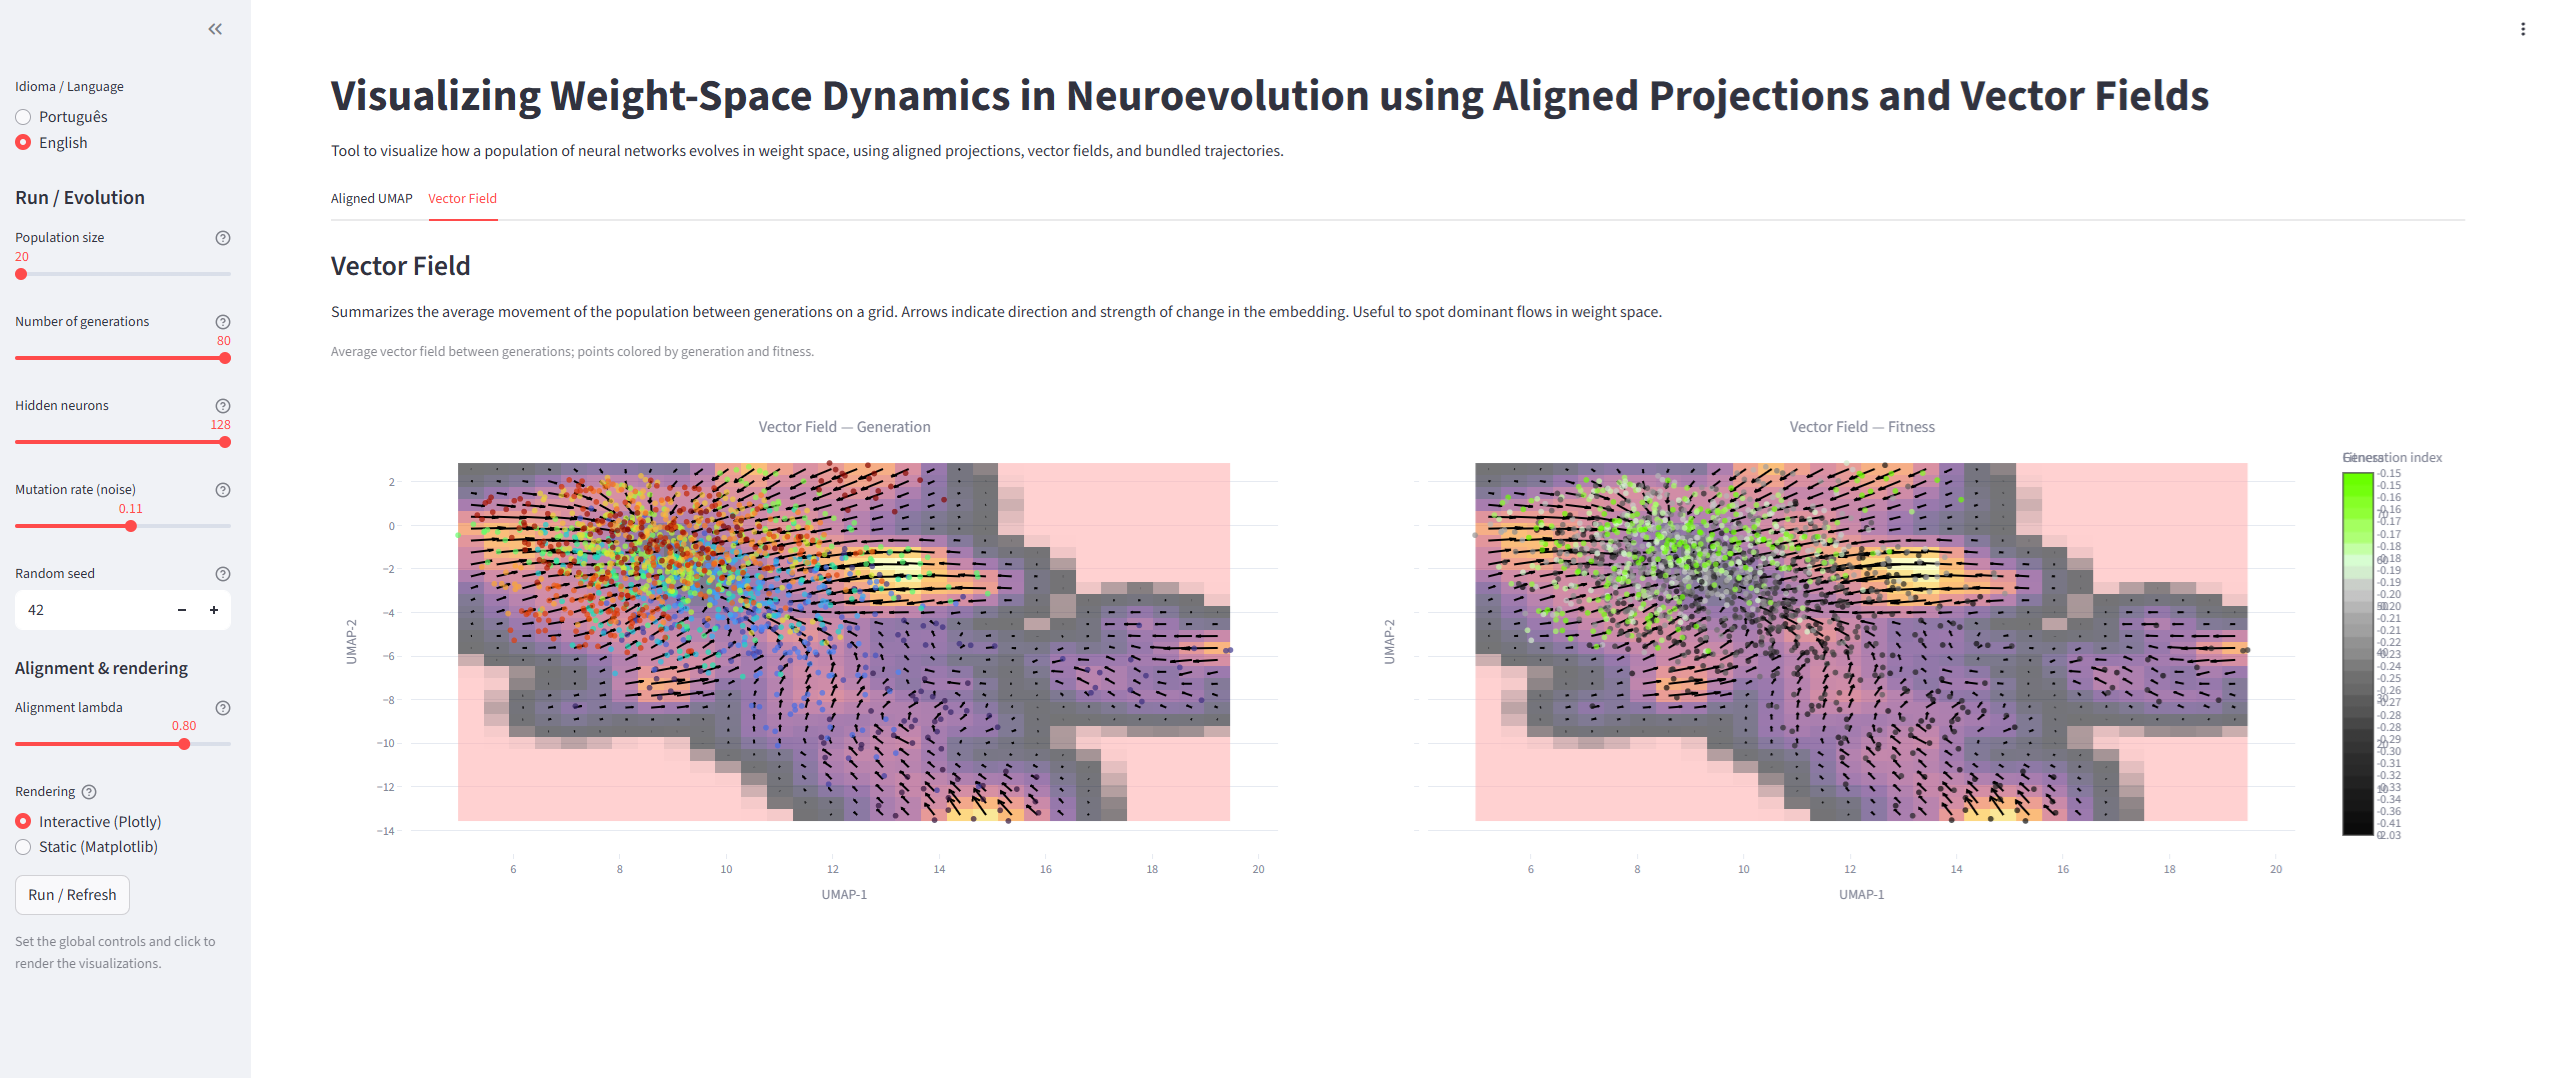
\includegraphics[width=0.9\linewidth]{streamlit6.png}

\end{frame}

\begin{frame}{Backup}

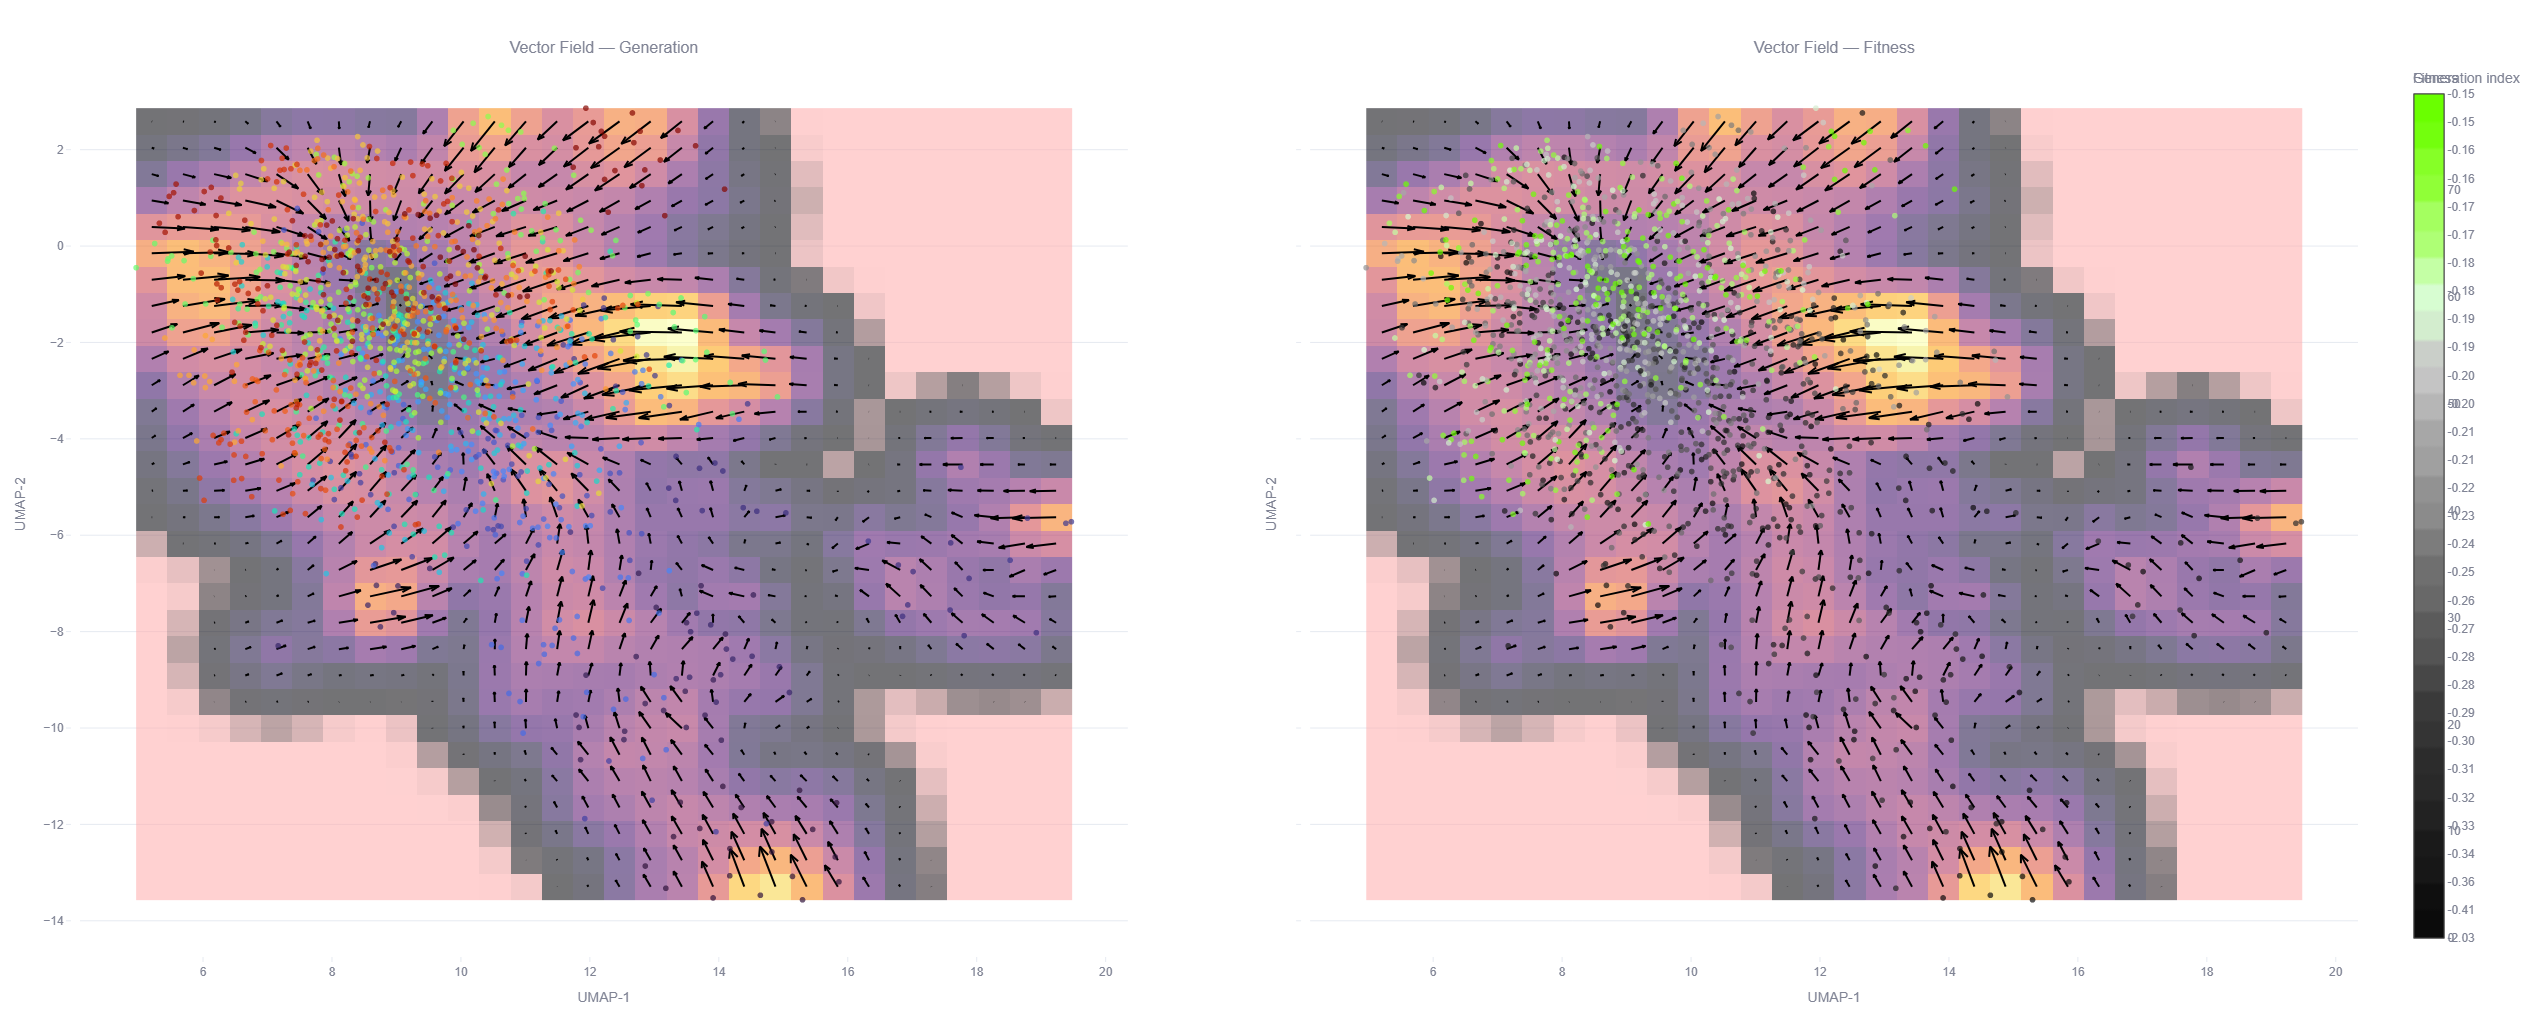
\includegraphics[width=0.9\linewidth]{streamlit7.png}

\end{frame}

\begin{frame}{Backup}

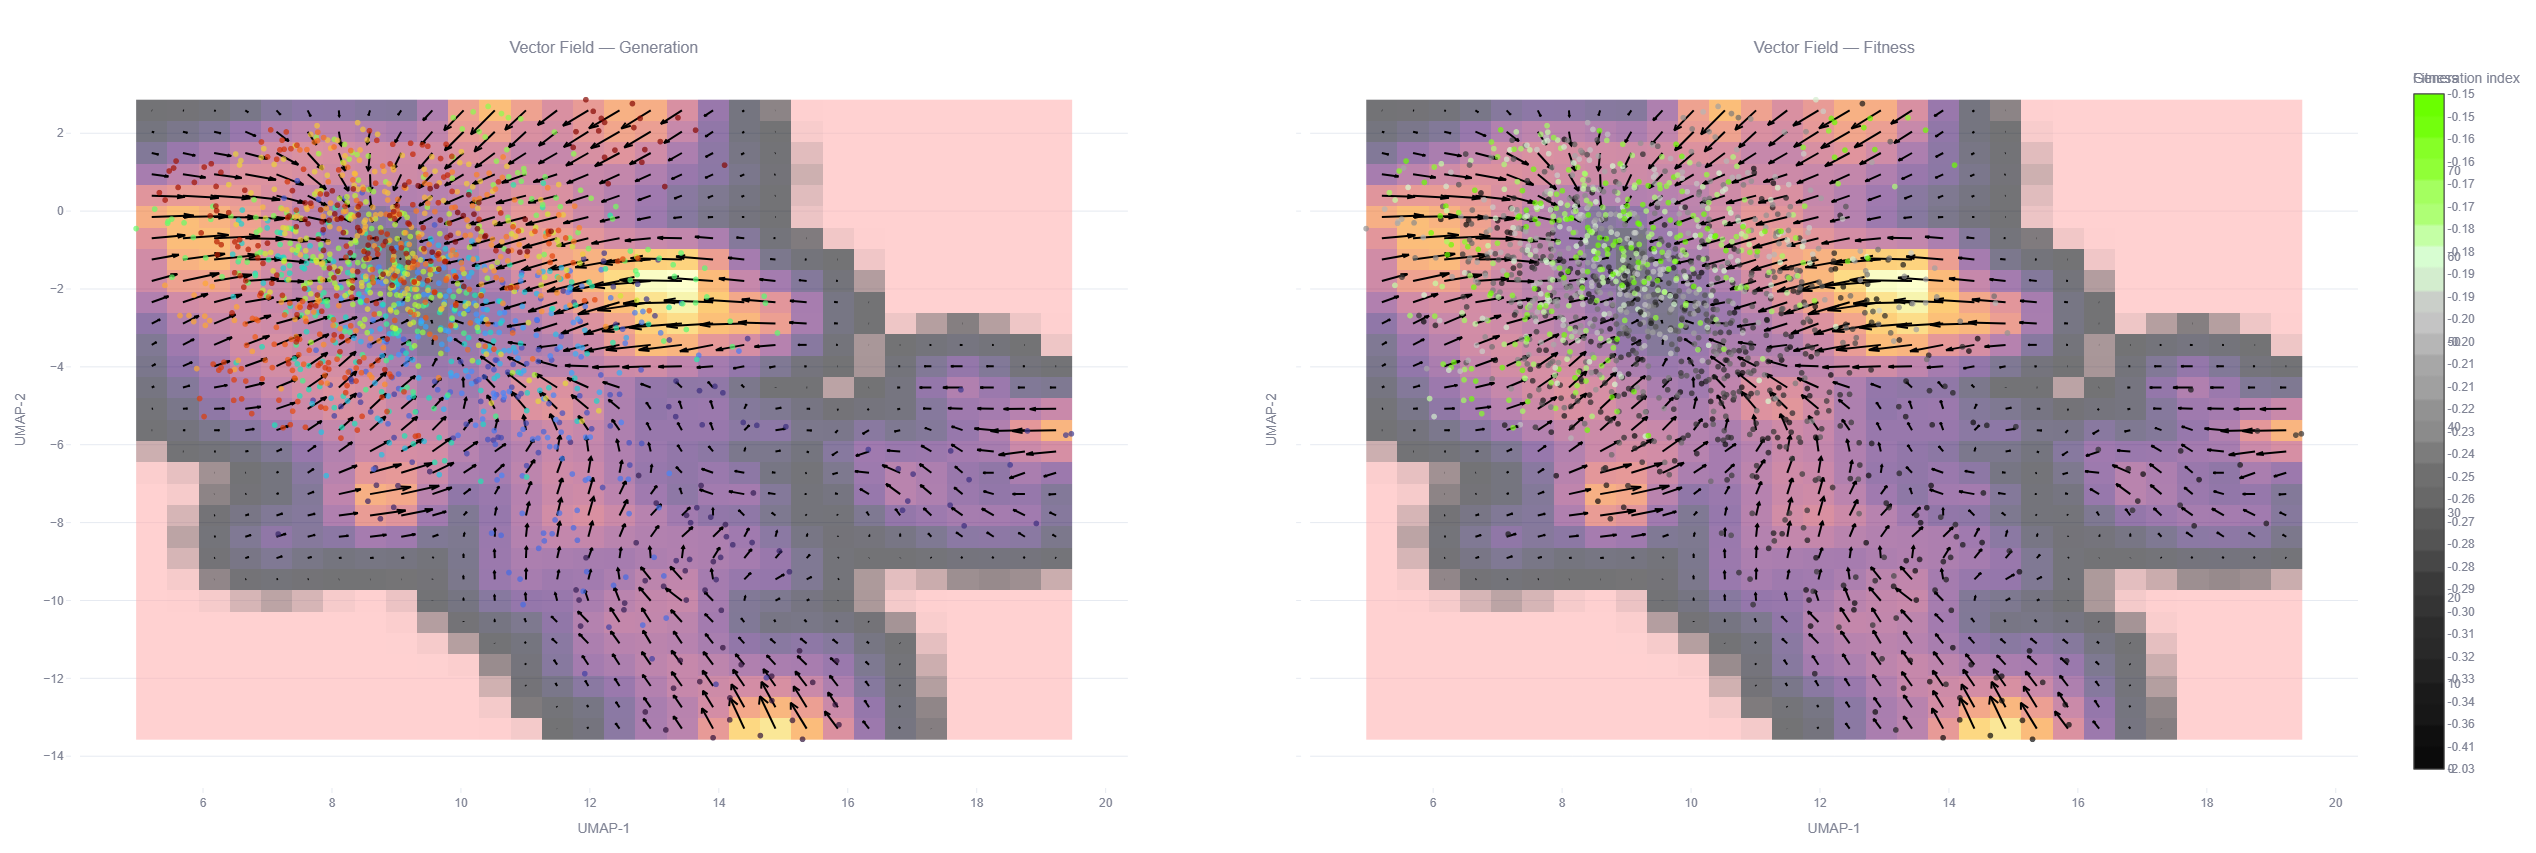
\includegraphics[width=0.9\linewidth]{streamlit8.png}

\end{frame}

\begin{frame}{Backup}

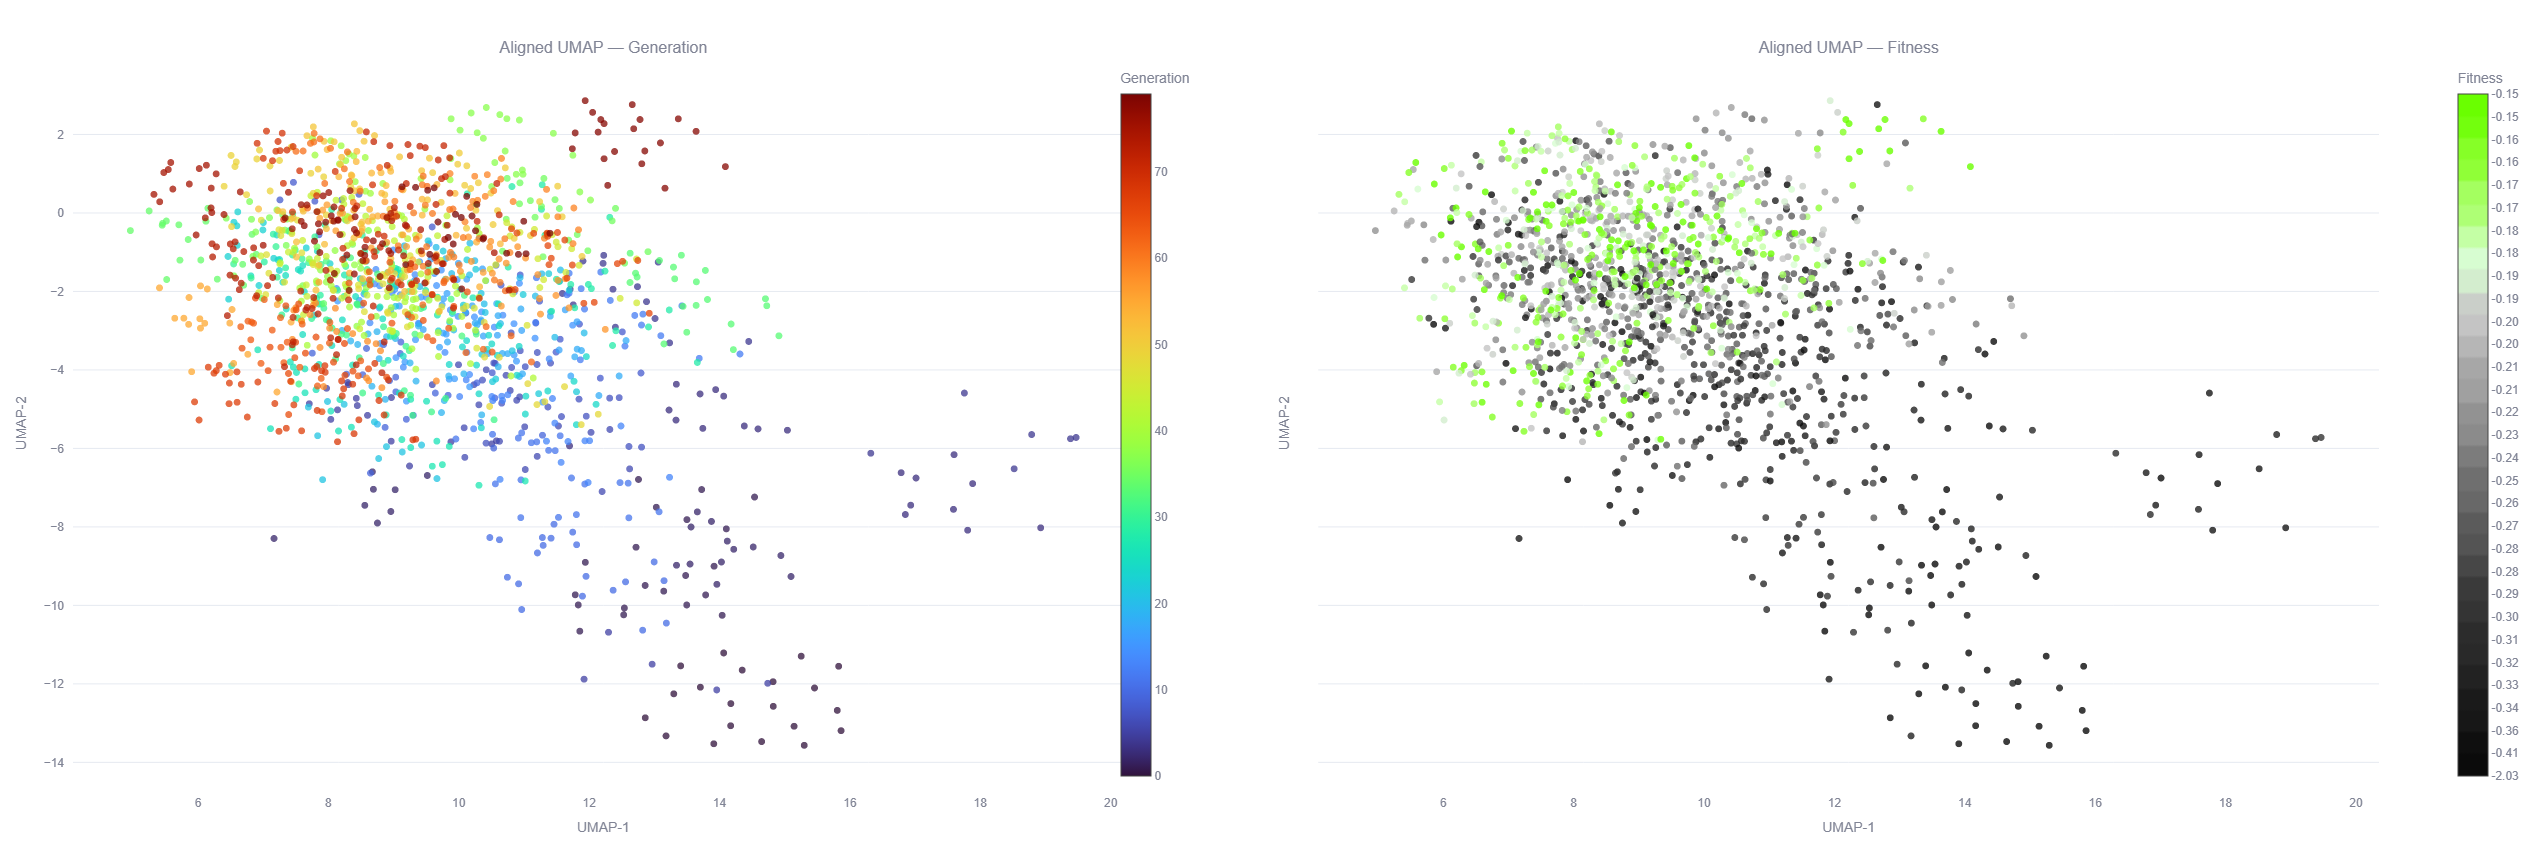
\includegraphics[width=0.9\linewidth]{streamlit9.png}





\end{frame}


\end{document}




